\documentclass{report}
\usepackage[dvipsnames]{xcolor}
\pagecolor{GreenYellow!10}
\usepackage[utf8]{inputenc}
\usepackage[spanish,mexico]{babel}
\setlength{\textwidth}{18cm}
\setlength{\oddsidemargin}{-1cm}
\setlength{\headsep}{-1cm}
\setlength{\voffset}{0cm}
\setlength{\topmargin}{0cm}
\setlength{\headheight}{0cm}
\usepackage{tikz}
\usetikzlibrary{calc,arrows}
\usepackage{multicol}
\usepackage{lipsum} 

\begin{document}

%%%%%% ENCABEZADO %%%%%%%%%%%%%%%%%%%%%%%%%%%%%%%%%%%%%%%
%\colorbox{white!10!}{
    \begin{minipage}[t]{0.165 \textwidth}
       \begin{flushright}
        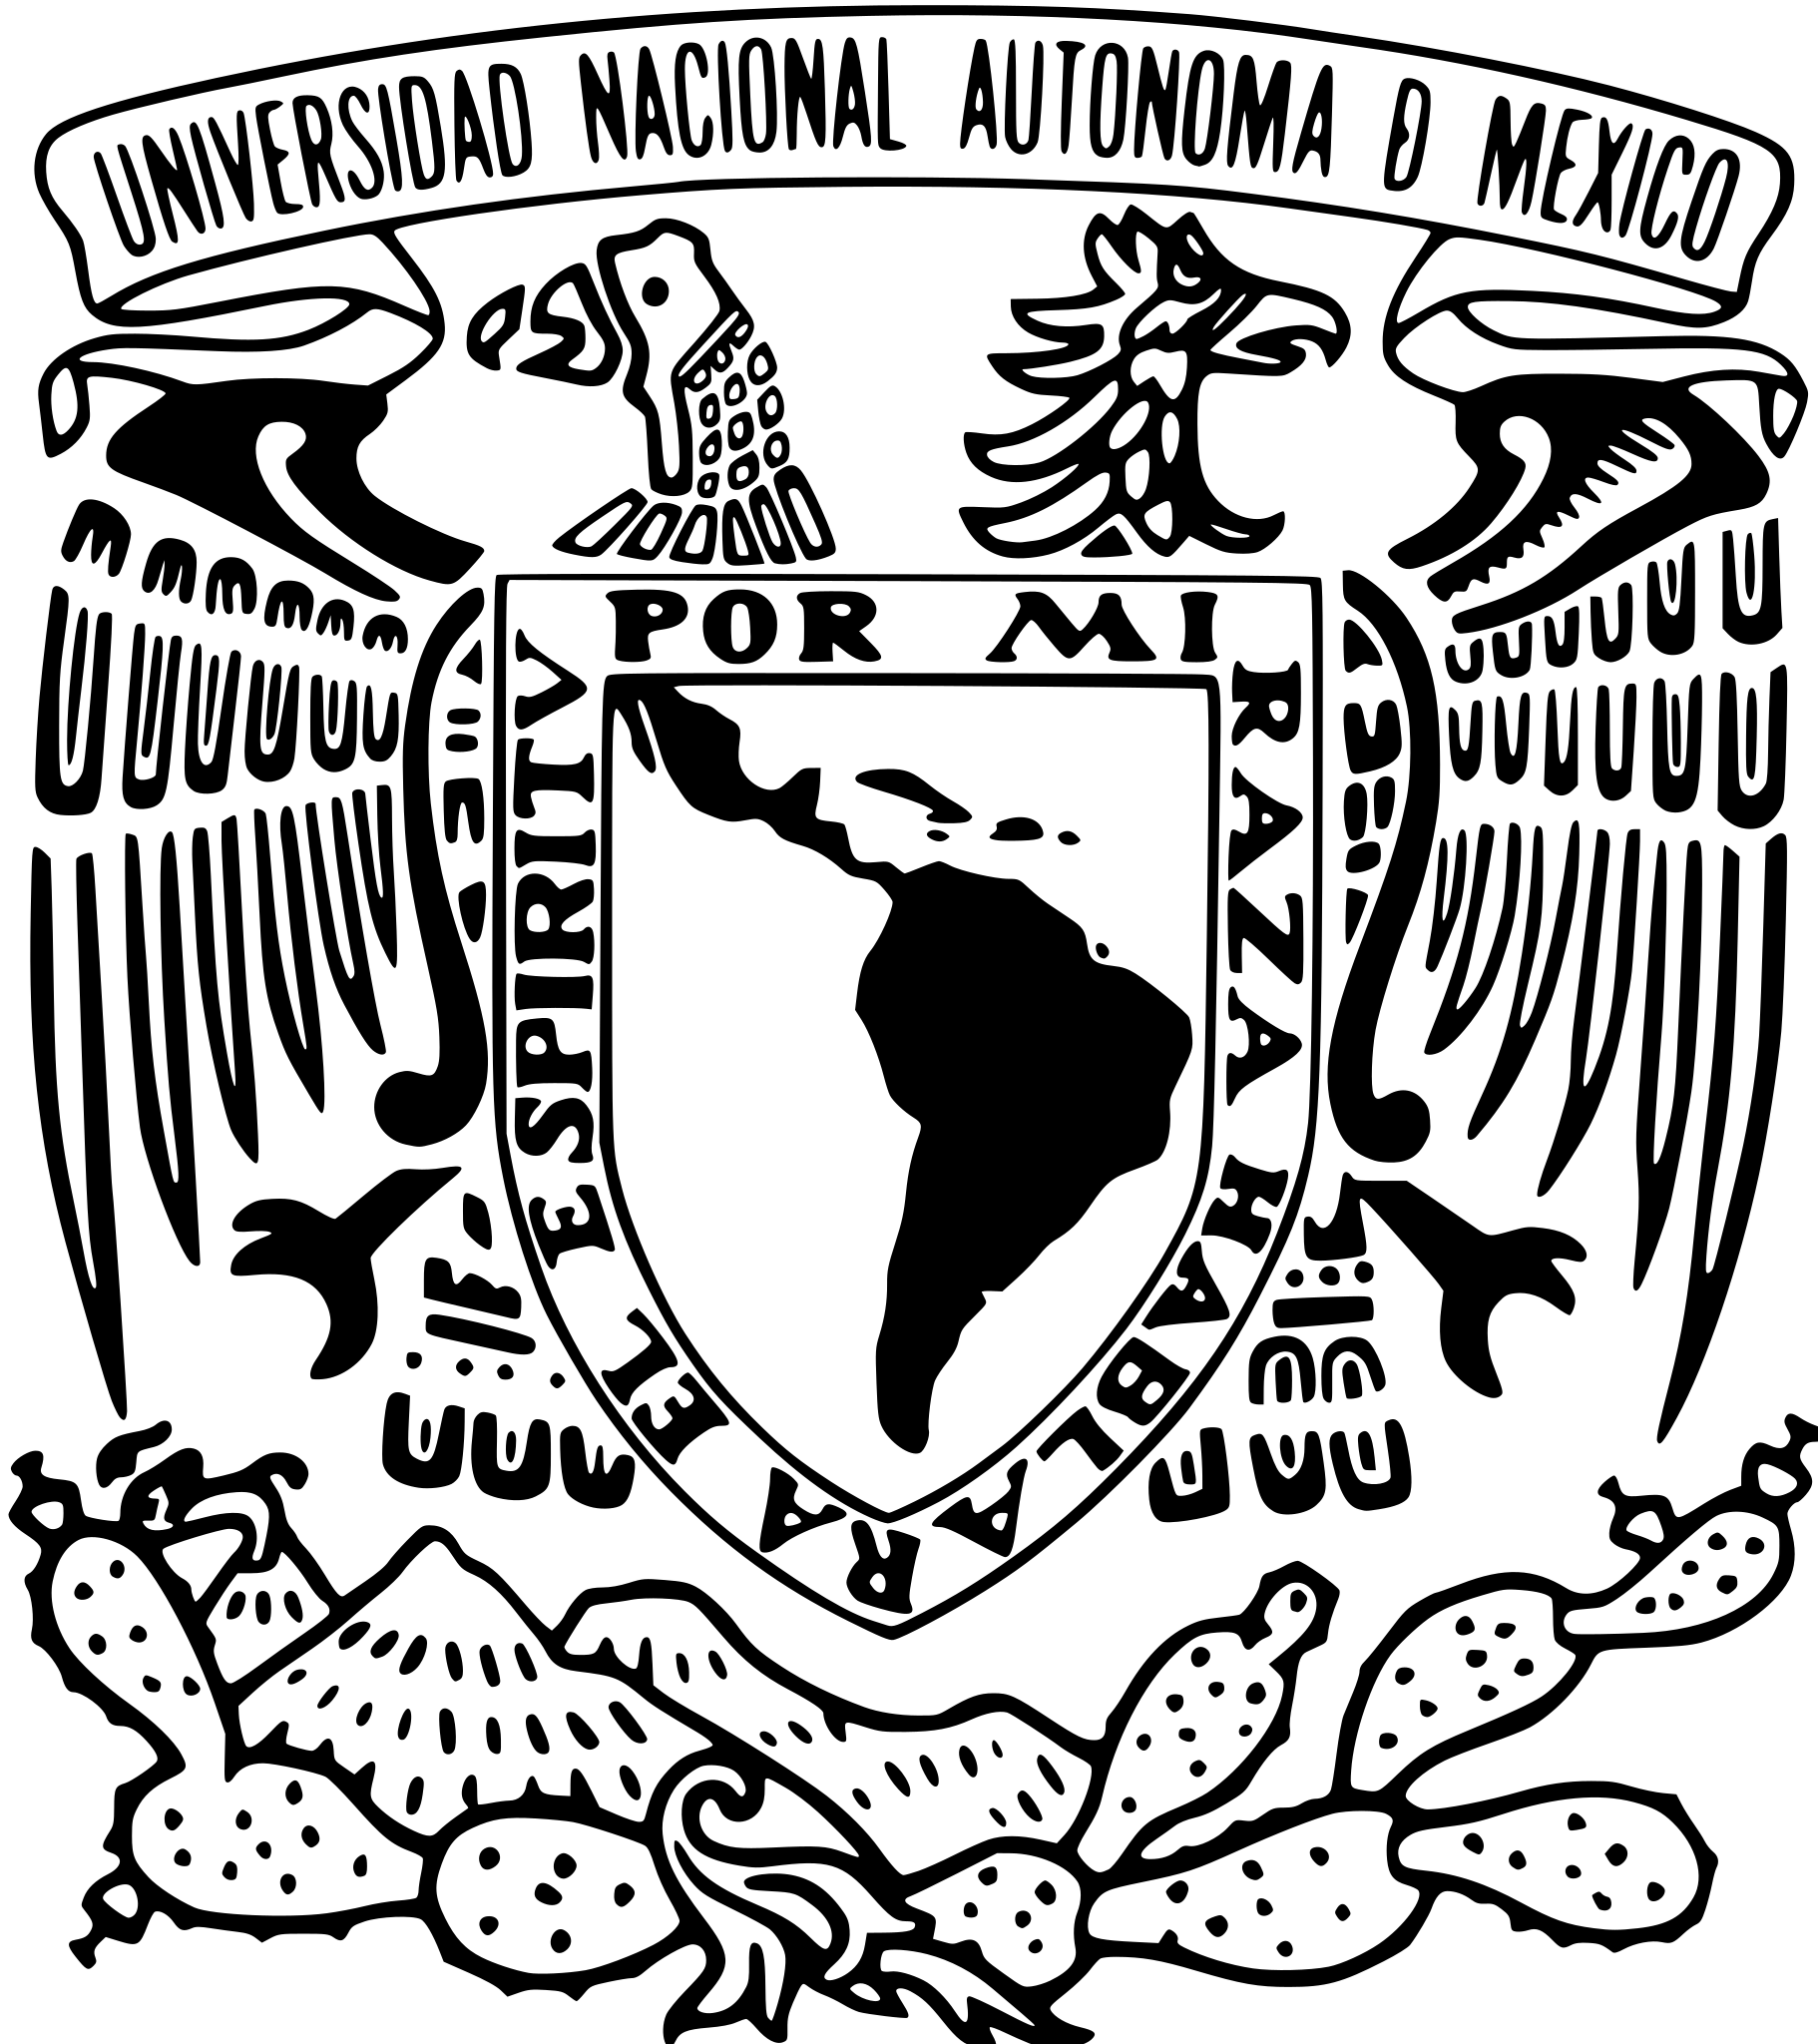
\includegraphics[width=1in]{EscudoUNAM.png}
       \end{flushright}
    \end{minipage}
    \begin{minipage}[H]{0.62 \textwidth}
        \begin{center}
            {\large \textsc{Universidad Nacional Autónoma de México}}
            \vspace{0.25cm}
            \\
            { \huge \textbf{Tarea 3}}
            \\
            \vspace{0.25cm}
            
            \textbf{Introducción a Ciencias de la Computación}
	    \\
	    \vspace{0.25cm}
	    \text{Rodrigo André Decuir Fuentes}
            \vspace{0.2cm}
        \end{center}
        \vspace{0.05cm}
    \end{minipage}
    \begin{minipage}[t]{0.165 \textwidth}
        \begin{flushleft}
            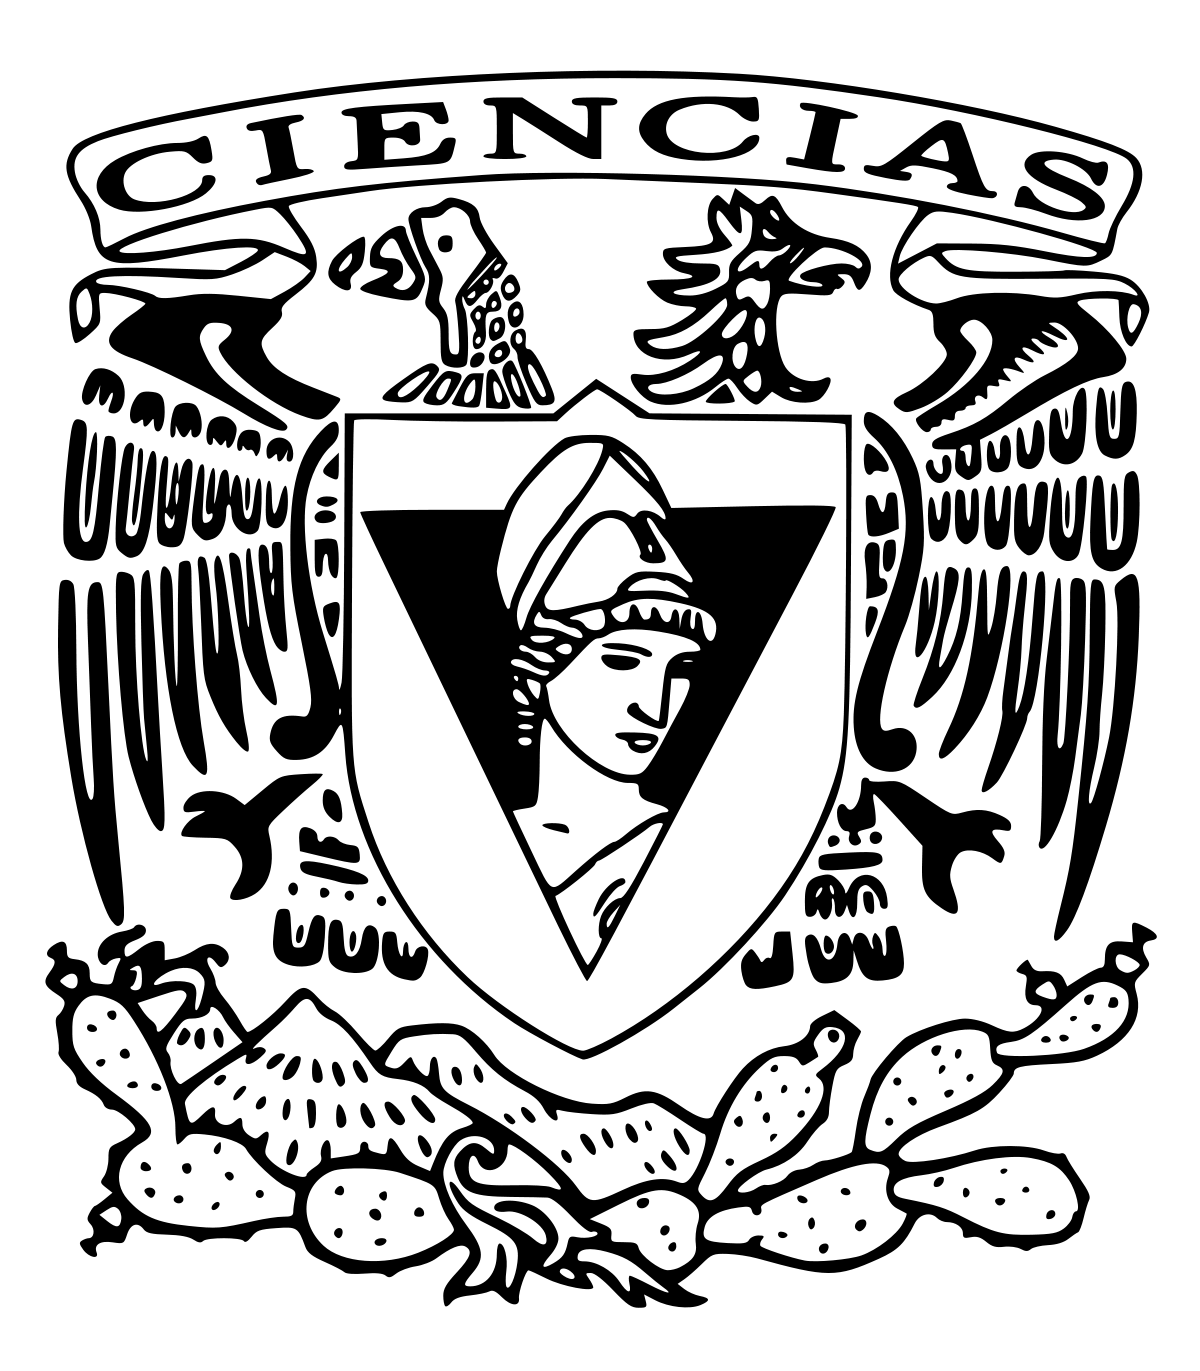
\includegraphics[width=1in]{Fciencias_UNAM.png}
        \end{flushleft}
    \end{minipage}
%}

\begin{tikzpicture}
    \draw[thick] (-6.5,0)--(11.2,0);
\end{tikzpicture}
%%%%%%%%%%%%%%%%%%%%%%%%%%%%%%%%%%%%%%%%%%%%%%%%%%%%%%%%%
\section*{Teoría}
\subsection*{Responde las siguientes preguntas:}
    \begin{enumerate}
	    \item \textbf{¿Que son los arreglos y para que son  ́utiles?}
	    	\begin{enumerate}
			\item Los arreglos son conjuntos finitos y ordenados de elementos homogéneos, asimismo son objetos.
            \item Son de mucha utilidad para manejar de forma sencilla y directa un conjunto de datos del mismo tipo. 
		    \end{enumerate}
	\item \textbf{¿Qué es la recursión y en qué se aplica? ¿Qué componentes debe tener un método recursivo?}
		\begin{enumerate}
			\item La recursión es la forma de expresar la solución a un problema en términos de sí mismo, es aplicada para trabajar en cosas que tienen muchas ramificaciones posibles y son demasiado complejas para un enfoque iterativo. Un buen ejemplo de esto sería buscar a través de un sistema de archivos. 
            \item Toda función recursiva tiene dos componentes: un caso base y un paso recursivo. 
		\end{enumerate}
	\item \textbf{¿Por que es tan importante la Complejidad en Ciencias de la Computación?}
		\begin{enumerate}
			\item Es importante porque nos permite determinar la eficacia de un algoritmo.
		\end{itemize}
	\item \textbf{A.I in Action, Robotics}
		\begin{itemize}
			\item Para cuestions prácticas, pensar se encuentra relacionado con hacer. De modo que los robots y la inteligencia artificial generan un patron en el intento de crear agentes autónomos que puedan funcionar en el mundo real. Los algoritmos y técnicas desarrollados permiten a la inteligencia artifical proveer pensamiento y planeación, en este sentido un robot provee la acción.
		\end{itemize}
	\item \textbf{Shakey}
		\begin{itemize}
			\item Shakey fue un robot móvil con cámaras y sensores de presencia, controlado por una gran computadora remota. Este robot fue un gran avance en visión computacional, procesamiento de lenguaje y planeación para entender instrucciones. Shakey fue el primer robot en pensar acerca de sus acciones, se probó mediante una serie de bloques y rampas.
		\end{itemize}
	\begin{center}	
		 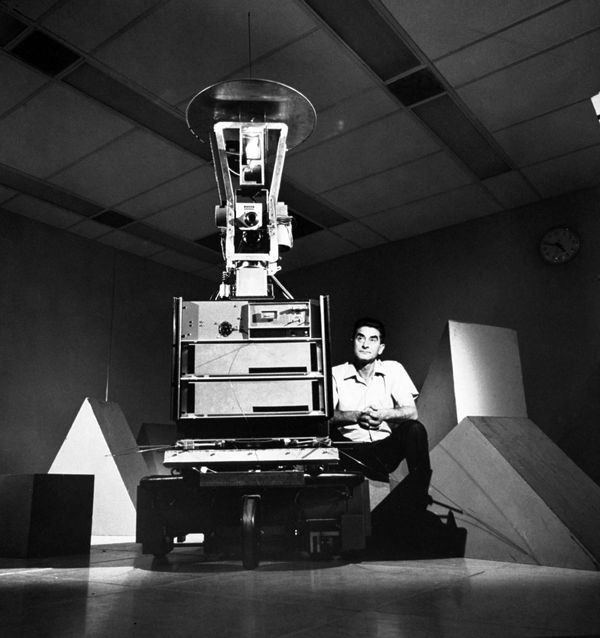
\includegraphics[width=0.6in]{shakey.jpg}
	\end{center}
	\item \textbf{Putting Robots to work}	
		\begin{itemize}
			\item En las fábricas los robots no parecen humanos, pues solo necesitan realizar su labor. Los robots industriales aparecieron una década después de las primeras computadoras. Al día de hoy la mayoría de los robots industriales son hechos en Japón.
		\end{itemize}
	\item \textbf{Robot Research}
		\begin{itemize}
			\item Las universidades han sido una gran fuente para la experimentación con robots. A partir de 1983 se comenzaron a vender robots autónomos.
		\end{itemize}
	\item \textbf{The Robots Around Us}
		\begin{itemize}
			\item Los robots pueden ser jugetes interesantes o herramientas muy serias. Aveces ambos. Y son fascinantes infinitamente. Su aparente comportamiento inteligente puede ser útil, provocativo y en algunos casos aterrador.
		\end{itemize}
    \end{enumerate}

\section*{Museo Nacional de Computación (TNMOC)}
\subsection*{Galería de Simulación}
\text{Esta galería se compone de un rango amplio de sistemas usados para simular algo.} 
	\begin{itemize}
		\item \textbf{Gray Supercomputers}
			\begin{itemize}
				\item El término 'Super Computación' data de 1920
				\item Fue hasta 1960 que el término 'Super Computadora' fue usado para referirse a computadoras muy rápidas
				\item Seymour Cray es uno de of pioneros de las 'super computadoras' entre 1960 y 1970
				\item La revolución de la super computación inició con el desarrolló de la CDC-6600, referida como una supercomputadora, la cual fue desarrollada por Cray y sus colegas durante su estancia en Control Data Corp (CDC), se vendieron 200 sistemas CDC-6600 cada uno por un precio de 9 millones de dolares
				\item En 1972 Cray inicia su propia compañía, Cray Research, la cuál dió lugar a las computadoras Gray
			\end{itemize}
		\item \textbf{INMOS Transputer}
			\begin{itemize}
				\item INMOS fue un compañía Británica fundada en 1978 
				\item INMOS diseñó sus propios microprocesadores (transputer)
				\item El sistema de desarrollo Transputer, permitió demostrar que se puede obtener mayor velocidad al usar más procesadores
			\end{itemize}
		\item \textbf{Analogue Computers}
			\begin{itemize}
				\item Antes de las computadoras digitales, existían las análogas, las cuales en lugar de usar binarios 0 y 1, usaban combinaciones de módulos fijados a voltajes con variables para crear circuitos que representaran problemas matemáticos
				\item La NASA fue de los primeros clientes de EAI(Electronic Associates Inc), compañía fundada en 1945, la cual empezó a manufacturar computadoras análogas en 1952
				\item La NASA utilizó las computadoras análogas para desarrollar pruebas espaciales y simular sistemas físicos
			\end{itemize}
		\item \textbf{Game Consoles}
			\begin{itemize}
				\item Al comenzar las computadoras a volverse más comerciales, comenzaron a aparecer computadoras dedicadas solo a jugar juegos. Entre dichos sistemas dedicados se encontraron los siguientes:
					\begin{itemize}
							
					\item Nintendo 64 - 1997
					\item Sega MegaDrive 2 - 1990
					\item Super Nintendo - 1992
					\item Atari 2600 - 1977

					\end{itemize}
			\end{itemize}
		\item \textbf{Arcade Games}
			\begin{itemize}
				\item Los juegos de Arcade se remontan a 1971 cuando el primer comercial de juegos fue producido. Los juegos de Arcade solo se volvieron comerciales cuando Atari lanzó Pong en 1972, uno de los primeros juegos basados en deporte. Luego con la evolución de la tecnología, nuevos juegos comenzaron a salir, entre ellos se encontraban los siguientes:
					\begin{itemize}
						\item  Crazy Taxi - Sega - 1999
						\item  Space Invaders - Taito - 1978
					\end{itemize}
			\end{itemize}
		\begin{center}
	          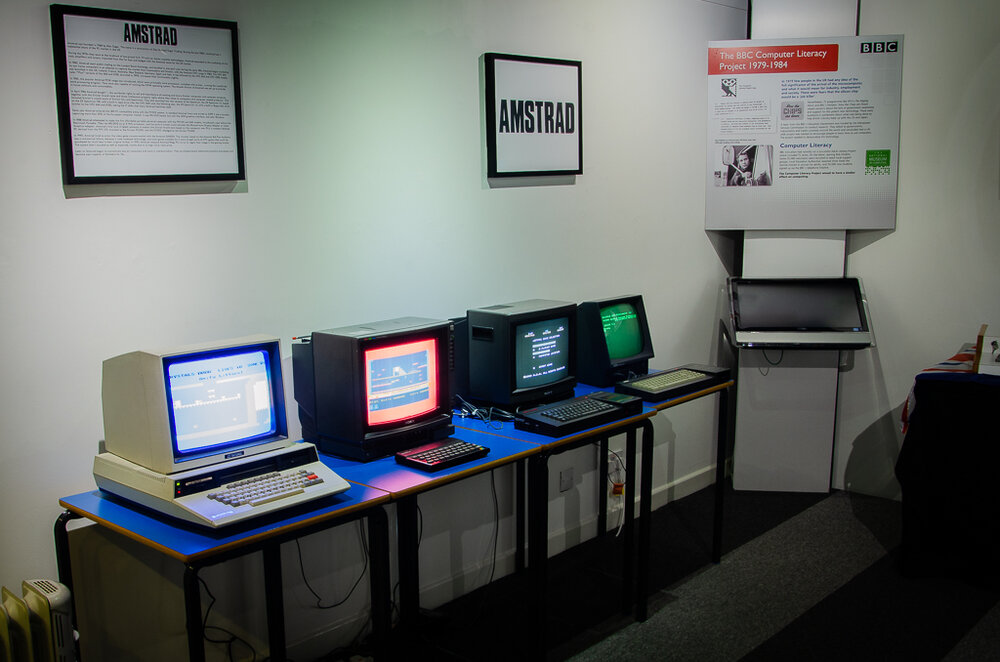
\includegraphics[width=1in]{space.jpg}
  		\end{center} 
		\item \textbf{PC Games}
			\begin{itemize}
				\item En el museo se tiene uno de los juegos más conocidos, DOOM
				\item Con la evolución de la tecnología los sistemas dedicados fueron remplazados por PCs modernas hasta el punto de que hoy en día los juegos de arcade usan una PC en lugar de hardware dedicado
			\end{itemize}
	\end{itemize}

\end{document}
